\documentclass[14pt]{extreport}
\usepackage[T1]{fontenc}
\usepackage[left=1in, right=1in, top=1in, bottom=1in]{geometry}
\usepackage{amsmath, amssymb, amsthm}
\usepackage{enumitem}
\usepackage{mathtools}
\usepackage{cancel}

% colored links
\usepackage{hyperref}
\hypersetup{
    colorlinks=true,
    linkcolor=blue,
    filecolor=magenta,      
    urlcolor=black!20!BurntOrange,
    }

% Inputting Python code
\usepackage[dvipsnames]{xcolor}
\definecolor{textblue}{rgb}{.2,.2,.7}
\definecolor{textred}{rgb}{0.54,0,0}
\definecolor{textgreen}{rgb}{0,0.43,0}
\usepackage{upquote}
\usepackage{listings}
\lstset{
    language=Python, 
    tabsize=4,
    basicstyle={\ttfamily},
    keywordstyle=\color{textblue},
    commentstyle=\color{textgreen},
    stringstyle=\color{textred},
    frame=none,
    columns=fullflexible,
    keepspaces=true,
    showstringspaces=false,
    xleftmargin=-15mm, % manual adjustment, figure out permanent solution
}

% Drawing figures
\usepackage{tikz}
\usetikzlibrary{matrix, positioning, shapes.geometric}
\usetikzlibrary{calc, shapes.symbols}

% Colored Boxes
\usepackage{tcolorbox}
\tcbuselibrary{skins,hooks}
\usetikzlibrary{shadows}
\usepackage{lipsum}

%Images
\usepackage{graphicx}
    \usepackage{subcaption}
    \usepackage{float}

%Formatting and Spacing
\setitemize[1]{noitemsep, parsep = 5pt, topsep = 5pt}
\setenumerate[1]{label = (\alph*), parsep = 1pt, topsep = 5pt}
\setlength\parindent{0pt}
\linespread{1.1}

%Stats
\newcommand{\Cov}{\text{Cov}}
\newcommand{\trace}{\text{trace}}
\newcommand{\Normal}{\text{Normal}}
\newcommand{\var}[1]{\operatorname{var}\left(#1\right)}
\newcommand{\E}[1]{\operatorname{E}\left[#1\right]}
\renewcommand{\Pr}[1]{\operatorname{P}\left(#1\right)}

%Custom Title Fields
\newcommand{\lectTitle}{Lecture 6 Notes}
\newcommand{\lectTime}{March 7, 2022}
\newcommand{\lectClass}{Advanced Algorithms}
\newcommand{\lectClassInstructor}{Dana Randall}
\newcommand{\lectSection}{Spring 2024}
\newcommand{\lectAuthorName}{Sarthak Mohanty}

\title{
    \vspace{1.75in}
    \textbf{\lectClass:\\ \lectTitle}\\
    \vspace{0.1in}\large{\textit{\lectClassInstructor\ \lectSection}}
    \vspace{2in}
    \author{\textbf{\lectAuthorName}}
    \date{}
}

\begin{document}

\maketitle
\pagebreak

\section*{Independence and Expectation}
    We will cover a few fundamental topics in probability as they apply to randomized algorithms: independence and expectation.

    \vspace{2mm}
    \textbf{Important: } A course in probability theory was a formal prerequisite for this class. Thus, although we are reviewing some concepts, we will assume basic knowledge of probability in this course. \href{https://www.dropbox.com/s/kov36bgyt286hqp/17-notes-mfml-probreview.pdf?dl=0}{This} set of lecture notes provides a concise review of concepts you should be familiar with.

    \begin{enumerate}[label=\arabic*.]
        \item The \textbf{expectation} of a function $g(X)$ of a continuous random variable with density $f_{X}(x)$ is $$\E{g(X)} = \int_{-\infty}^{\infty} g(x) f_{X}(x)\ dx.$$ Can be considered as ``average" value. It is also true that $$\E{g_{1}(X) + g_{2}(X)} = \E{g_{1}(X)} + \E{g_{2}(X)}:$$ this property is known as \textbf{linearity of expectation}.
        \item We call two random variables $A$ and $B$ \textbf{independent} if $$\Pr{A = a, B  = b} = \Pr{A = a}\Pr{B = b}.$$ Similarly, we call two events independent if $$\Pr{A \cap B} = \Pr{A} \times \Pr{B}$$
        When discussing a collection of events or random variables, \( \{X_i\}_{i}^{n} \), they are said to be \textbf{$k$-wise independent} if every subset of size at most $k$ is mutually independent.
    \end{enumerate}

\subsection*{Multiparty Computation}
    Consider the following problem. There are $N$ students in this course who wish to determine the average score on the midterm. However, none of them want to reveal their own scores. Even if $k$ of the $N$ "friends" are dishonest, then they should still learn no more than the sum of the remaining $N - k$ honest ones (which they can figure out anyway from the answer). 

    \vspace{2mm}
    Let's formalize the above statement. Say we have $N$ people, each person $i$ has a secret $S_{i}$. Let $m = 101 \cdot N$. If $0 \le S_{i} \le 100$, then $m = 101 \cdot N > \sum_{i}S_{i}$. 

    \vspace{2mm}
    Person $i$: 
    \begin{enumerate}[label=\arabic*.]
        \item Picks random variables $X_{i1}, \dots, X_{iN - 1}$.
        \item Sets $X_{iN} = y_{i} = S_{i} - (X_{i1} + X_{i2} + \dots + X_{iN - 1}) \pmod{m}$.
        \item Distributes the $N - 1$ random variables to the others (one per person) and keeps $Y$.
    \end{enumerate}
    Once this process is complete for all players, each player announces his result $\pmod{m}$. Then, the sum of each of the announced results is the desired sum $S$.

    \vspace{2mm}
    An illustration of the protocol is shown below. Hopefully by looking at the values in the table, it can be seen the sum is correct. But, it remains to determine the security of the algorithm.

\begin{figure}[htbp]
    \centering
    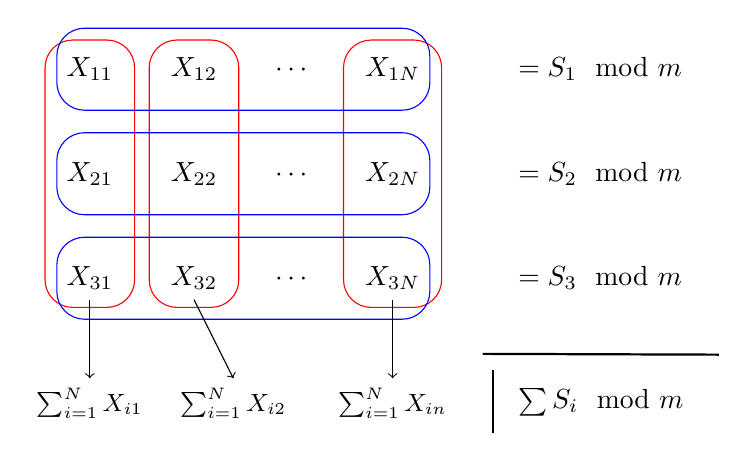
\begin{tikzpicture}
        \matrix (m) [matrix of math nodes, column sep=0.5cm, row sep=0.8cm]
        {
        X_{11} & X_{12} & \cdots & X_{1N} \\
        X_{21} & X_{22} & \cdots & X_{2N} \\
        X_{31} & X_{32} & \cdots & X_{3N} \\
        };
        
        % Drawing ovals around columns
        \foreach \i in {1,2,4}
        {
        \draw [rounded corners=10, color=red] ([xshift=-1.5mm, yshift=1mm]m-1-\i.north west) rectangle ([xshift=1.5mm,yshift=-1mm]m-3-\i.south east);
        }
        
        % Drawing ovals around rows
        \foreach \i in {1,2,3}
        {
        \draw [rounded corners=10, color=blue] ([yshift=2.5mm]m-\i-1.north west) rectangle ([yshift=-2.5mm]m-\i-4.south east);
        }
        
        % Adding equal signs and expressions next to each row
        \foreach \i in {1,2,3}
        {
        \node [right=of m-\i-4] {$= S_{\i} \mod m$};
        }
        
        % Drawing arrows and sum expressions for columns
        
        \draw [->] (m-3-1.south) -- +(0,-1cm);
        \node [below=1cm of m-3-1.south] {\small$\sum_{i=1}^{N} X_{i1}$};
        
        \draw [->] (m-3-2.south) -- +(5mm,-1cm);
        \node [below=1cm of m-3-2.south, xshift=5mm] {\small$\sum_{i=1}^{N} X_{i2}$};

        \draw [->] (m-3-4.south) -- +(0,-1cm);
        \node [below=1cm of m-3-4.south] {\small$\sum_{i=1}^{N} X_{in}$};
        
        % Adding the sum of S_i mod m at the bottom right
        \node [below right=of m-3-4, anchor=north west] (sum) {$\sum S_{i} \mod m$};
        
        
        % Draw a horizontal line to the left of the sum
        \draw [-, thick] ([xshift=-0.2cm,yshift=0.4cm]sum.west) -- ([xshift=-0.2cm,yshift=-0.4cm]sum.west);
        % Draw a vertical line above the sum
        \draw [-, thick] ([xshift=-1.5cm,yshift=0.31cm]sum.north) -- ([xshift=1.5cm,yshift=0.3cm]sum.north);
    \end{tikzpicture}
        \caption{Diagram of each of the $X_{i}$s}
        \label{fig:enter-label}
    \end{figure}
    Some useful facts:
    \begin{itemize}
        \item Say $X$ is a random variable uniformly distributed in $S = \{0, 1, \dots, m-1\}$.  Then, clearly for any fixed $a$, the variable $Y = X + a \pmod{m}$ is also uniform in $S$ (though $X$ and $Y$ are dependent).
        \item If $X_1, \dots, X_k$ are independent r.v's uniform in S and Y is defined to be $a - (X_1 + ... X_k) \pmod{m}$ for some fixed a, then these $k+1$ r.v.s are k-wise independent. Just check that $\Pr{Y = y | X_2 = x_2, X_3 = x_3, ..., X_k = x_k} = 1/m$.
    \end{itemize}
    Claim is secure in following sense: for any set of $t$ honest players, only information that the rest of players have, even if they cheat, is the sum of the t players' values.  What does this really mean?  What is "information"?  What we mean is that if you modify the values for these players keeping the sum the same, then the probability distribution on the sequence of outputs produced by those players doesn't change.  
    
    
    \vspace{5mm}
    \textbf{Proof.} Consider the t all sent their $Y$ value to the same honest player.  (Doesn't change protocol).  For any fixed sequence of coin tosses, all sets of $t$ values with the same sum lead to exactly the same information revealed to the other players.  So, all sets with the same sum have the same distribution.


\subsection*{Gambler's Problem}
    Consider a casino where are games are fair and the expected value of all games is zero, i.e. $\Pr{W} = \Pr{L} = \frac{1}{2}$. Intuitively, we know we cannot game this system. But, it's a good exercise to convert our intuition to a formal proof.

    \vspace{2mm}
    Define $X_{i}$ to be the gain at time $i$. So $X = X_{1} + \dots + X_{N}$ where $N$ is \# seconds in a day. Let $p_{ij}$ be the probability that we bet $j$ at time $i$. So $$\E{X_{i}} = \sum_{j} \frac{j \cdot p_{ij}}{2} - \frac{j \cdot p_{ij}}{2} = 0,$$ and by linearity of expectations, we have $$\E{X} = \E{\sum_{i = 1}^{N} X_{i}} = \sum_{i = 1}^{N}\E{X_{i}} = 0$$

    \textbf{Exercise. } You are playing a special game of cards against Professor Randall. Each turn, she flips over a card. You are allowed, at any time, to predict the next card will be red. If it is indeed red, you get 1 pt. If it is black, Professor Randall gets one point. Is there a strategy you can use to gain an advantage (in expectation?) Answer is \textbf{No.}
    
\subsection*{Randomized 3-SAT}
    One fundamental application of randomized algorithms is in the \textsf{MAX-Exact-3-SAT} problem, an NP-complete problem. 
    \begin{tcolorbox}
        The \textsf{MAX-Exact-3-SAT} problem is a variant of the well-known 3-SAT problem. Given a boolean formula in CNF: $$\phi = C_{1} \land C_{2} \land \dots \land C_{n},$$ where each clause contains \textit{exactly} three literals, the \textsf{MAX-Exact-3SAT} problem seeks the truth assignment that maximizes the number of satisfied clauses.
    \end{tcolorbox}
    \vspace{5mm}
    \textbf{Proposition. } Given an input of \textsf{MAX-Exact-3SAT}, a random assignment will satisfy at least 87.5\% of the clauses in expectation.

    \vspace{5mm}
    \textbf{Proof.} Let $S$ be the random variable denoting the number of satisfied clauses with a random assignment. Let $S_{i}$ be the indicator random variable denoting whether or not clause $i$ evaluates to True, for $1 \le i \le n$. Define $S$ and $S_{i}$ as above. Now
    $$\begin{aligned}
        \E{S_{i}} &= \Pr{\bigcup_{j = 1}^{3} \text{(literal $j$ evaluates to True)}} \\
        &= 1 - \Pr{\text{no literals evaluate to True}} \\
        &= 1 - \left(\frac{1}{2}\right)^{3} \\
        &= \frac{7}{8} = .875.
    \end{aligned}$$
    Using the linearity of expectations, we conclude $$\E{S} = \sum_{i = 1}^{n}\E{S_{i}} = .875n.$$ This problem is especially interesting because this simple randomized algorithm gives a $7/8$-approximation. Moreover, this guarantee is essentially optimal: for every constant $\varepsilon > 0$, a polynomial-time algorithm that always achieves a $(7/8 + \varepsilon)$-approximation for \textsf{MAX-Exact-3-SAT} would imply $\textsf{P} = \textsf{NP}$.
     
         

    % Practice Problem: Show that for \textsc{Max-Exact-3SAT}, if there is an assignment that satisfies strictly less than 87.5\%  of clauses, then there is another assignment that satisfies stricly more than 87.5\% of the clauses.
    % Practice Problem: Give an example of an input of \textsc{MAX-Exact-3SAT} such that every assignment satisfies exactly 87.5\% of the clauses.
    
    
    % solution:
        % Define $S$ as above. Now suppose there is an assignment that satisfies strictly less than 87.5\% of the clauses. Note that we can alternatively define $\E[S]$ as $$\E[S] = \frac{1}{n}\sum_{i = 1}^{n} (\text{\% of clauses satisfied by assignment $i$}),$$ where $n$ in this case is the number of distinct assignments. If all other assignments satisfied at most 87.5\% of the clauses, then $$\frac{1}{n}\sum_{i = 1}^{n} (\text{\% of clauses satisfied by assignment $i$}) < 87.5\%.$$ But from part $b$, we know $\E[B] \ge 87.5\%$. This would be a contradiction, therefore there is another assignment that satisfies strictly more than 87.5\% of the clauses.
        % Can we turn this idea into a 7/8-approximation algorithm? In general, a random variable can almost always be below its mean.
        % \item $$(x_{1} \lor x_{2} \lor x_{3}) \land (x_{1} \lor x_{2} \lor \neg x_{3}) \land (x_{1} \lor \neg x_{2} \lor x_{3}) \land (x_{1} \lor \neg x_{2}\lor \neg x_{3}) $$
        % $$\land (\neg x_{1} \lor x_{2} \lor x_{3}) \land (\neg x_{1} \lor x_{2} \lor \neg x_{3}) \land (\neg x_{1} \lor \neg x_{2} \lor x_{3}) \land (\neg x_{1} \lor \neg x_{2} \lor \neg x_{3})$$

\end{document}